\documentclass[14pt,aspectratio=169]{beamer}
\usetheme{Marburg}
\graphicspath{{Arquivos/}}
\usepackage[utf8]{inputenc}
\usepackage[portuguese]{babel}
\usepackage[T1]{fontenc}
\usepackage{amsmath}
\usepackage{amsfonts}
\usepackage{amssymb}
\usepackage{graphicx}
\author{C Shruti EE18BTECH11006}
\newcommand{\TT}{EE2227 Control Systems}
\newcommand{\TB}{Gate Problems}
\newcommand{\DT}{IIT Hyderabad 12-2-2020}
\newcommand{\IN}{-->}
\newcommand{\PI}{I - Question}
\newcommand{\PII}{II - Theory required}
\newcommand{\PIII}{III - Solution}

\title{\TT}
%\setbeamercovered{transparent} 
\setbeamertemplate{navigation symbols}{\href{www.egmon.com.br}{www.egmon.com.br}} 
\logo{\includegraphics[scale=0.033]{LogoReformada}} 
\institute{IIT Hyderabad} 
\date{12-02-2020} 
%\subject{} 
\begin{document}

\section{\PI}
\section{\PII}
\section{\PIII}
\begin{frame}
\titlepage
\pause
\Large
 GATE-2019, EE Section 
 \newline Problem no.13
\end{frame}


\section{\DT}
\begin{frame}{\TB}{\TT}
 
13)  The output response of a system is denoted as y(t), and its Laplace transform is given by 

Y(s) = \dfrac{10}{s(s^2+ s + 100{(2)^{0.5})}}

The steady state value of y(t) is 

a) 100(2)^{0.5}\hspace{4cm}
b) \dfrac{1}{10(2)^{0.5}}\linebreak
c)  10(2)^{0.5} \hspace{4cm}
d) \dfrac{1}{100(2)^{0.5}}\linebreak

\end{frame}

\begin{frame}{\TB}{\TT}


\begin{figure}[htp]
    
    The final value theorem states that  \[ \lim_{t \to \infty} y(t) = \lim_{s \to 0} sY(s)\]
\newline This is valid only when sY(s) has poles that lie in the negative half of the real side.
\end{figure}
 
\end{frame}

\begin{frame}{\TB}{\TT}
 
  If the quadratic equation $ax^2 + bx + c$ has complex roots then the real part of those roots will be -b/2a
  
  Hence, verified that the roots of $s^2+ s + 100{(2)^{0.5}}$ have a negative real part which is -0.5. So, Final value theorem is applicable.
 
\end{frame}
\begin{frame}{\TB}{\TT}
 \begin{block}{Solution:(b)}
 Steady state value of y(t) = \[ \lim_{t \to \infty} y(t) = \lim_{s \to 0} sY(s) = \lim_{s \to 0} \dfrac{10s}{s(s^2+ s + 100{(2)^{0.5})}} \]   
 \centering
 = \dfrac{10}{100(2)^{0.5}} =  \dfrac{1}{10(2)^{0.5}}
\end{block}
\end{frame}

\begin{figure}[htp]
    \centering
    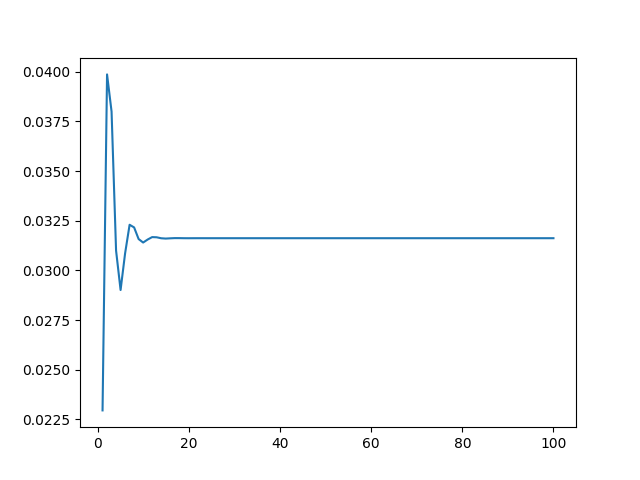
\includegraphics[width=8cm]{shru1.png}
    \caption{ y(t)}
    \label{steady state}
We can see that y(t) is approaching a constant value 0.031 which is verifies our answer!
    
\end{figure}
\begin{frame}




 

\large
\centering
Thank You!


\end{frame}
\end{document}
